\documentclass[10pt,twocolumn]{article}
\usepackage{graphicx}
\usepackage[bottom=1.5cm, right=1cm, left=1cm, top=1cm]{geometry}

\usepackage{amsmath, amsthm, amsfonts, amssymb}
\usepackage[utf8]{inputenc}
\usepackage[T2A]{fontenc}
\usepackage[english, russian]{babel}

\usepackage{import}
\usepackage{pdfpages}
\usepackage{transparent}
\usepackage{xcolor}

\usepackage{parskip}
\usepackage{systeme}

\newcommand{\incfig}[2][1]{%
    \def\svgwidth{#1\columnwidth}
    \import{./figures/}{#2.pdf_tex}
}

\pdfsuppresswarningpagegroup=1

\usepackage{hyperref}
\hypersetup{
    colorlinks=true, %set true if you want colored links
    linktoc=all,     %set to all if you want both sections and subsections linked
    linkcolor=black,  %choose some color if you want links to stand out
}

\newcommand\hr{
    \noindent\rule[0.5ex]{\linewidth}{0.5pt}
}

% All the environments
\usepackage{mdframed}
\mdfsetup{skipabove=1em,skipbelow=0em}
\theoremstyle{definition}
\newmdtheoremenv[nobreak=true]{theorem}{Теорема}
\numberwithin{theorem}{section}
\newmdtheoremenv[nobreak=true]{lemma}{Лемма}
\numberwithin{lemma}{section}
\newmdtheoremenv[nobreak=true]{definition}{Определение}
\numberwithin{definition}{section}
\newmdtheoremenv[nobreak=true]{corollary}{Следствие}
\numberwithin{corollary}{section}
\newtheorem*{eg}{Пример}
\newtheorem*{remark}{Замечание}

\numberwithin{equation}{section}

% Defs
\let\phi\varphi
\let\epsilon\varepsilon
\let\kappa\varkappa
\let\implies\Rightarrow
\let\iff\Leftrightarrow
\let\true\hookrightarrow

\newcommand{\pd}[2]{\frac{\partial{#1}}{\partial{#2}}}
\newcommand{\pdd}[2]{\frac{\partial^2{#1}}{\partial{#2^2}}}
\newcommand{\pdm}[3]{\frac{\partial^2{#1}}{\partial{#2}\partial{#3}}}
\newcommand\R{\ensuremath{\mathbb{R}}}


\begin{document}

\section{Геом оптика}
\begin{gather*}
  \frac{\sin \alpha}{\sin \beta}=\frac{n_2}{n_1} \qquad n = \sqrt{\epsilon}
\end{gather*}
В оптически более плотной среде (n больше), угол меньше.
\begin{gather*}
  \frac{1}{F}=(\frac{n_2}{n_1}-1)(\frac{1}{R_1}+\frac{1}{R_2}) \\ \frac{1}{b}+\frac{1}{d}=\frac{1}{F} \qquad \Gamma_{\parallel} = \Gamma_{\perp}
\end{gather*}
Здесь у линзы $n_2$ у среды $n_1$. В случае различных n слева и справа: $f'/f=n'/n$
\[
  R_E=(\frac{n_1-n_2}{n_2+n_1})^2
\]
Предельные угол: $\alpha = \arcsin \frac{n_2}{n_1}$
\subsection{Радиус кривизны}
\begin{gather*}
  R = \frac{1}{k} \qquad k = \frac{|x'y''-x''y'|}{\sqrt{x'^{2}+y'^{2}}^{3}} \qquad k=\frac{|f''|}{\sqrt{(1+f'^{2})^{3}}} \\ 
  k = \sqrt{\frac{(y'z''-y''z')^{2}+(x'z''-x''z')^{2}+(x'y''-x''y')^2}{(x'^{2}+y'^{2}+z'^{2})^{3}}}
\end{gather*}
\section{Уравнение волны}
\begin{gather*}
  \xi = a \cos \omega (t - x/v) \qquad v = \lambda \nu \qquad k=2\pi/\lambda \\ 
  \pd{\xi}{x}=\pm \frac{1}{v}\pd{\xi}{t} \qquad \frac{\partial^{2}\xi}{\partial x^{2}}=\frac{1}{v^{2}}\frac{\partial^{2}\xi}{\partial t^{2}} \\ 
  v = \sqrt{\frac{E}{\rho}} \qquad v = \sqrt{\frac{\gamma RT}{\mu}}
\end{gather*}
$\mu$ - молярная масса, $R=8.31$, постоянная Больцмана $k=1.38 \cdot 10^{-23}$ Дж/К

Стоячая волна: $\xi=\xi_1+\xi_2=A\cos (kx) \cdot \cos (\omega t)$, $A = 2a$,
где $\xi_1$ и $\xi_2$ направлены в разные стороны 
Для звука: 
\[
  R_E=(\frac{\rho_1c_1 - \rho c}{\rho_1c_1 + \rho c})^{2}
\]
\section{Эффект доплера}
\begin{gather*}
  \nu'=\nu\frac{v-u_x'}{v-u_x}
\end{gather*}
$u_x'$ и $u_x$ - проекции скоростей приёмника и источника на ось совпадающую
с направлением распространения импульсов
\section{Интерференция}
\begin{gather*}
  x_m = \frac{m\lambda l}{d} \qquad \Delta x = \frac{\lambda l}{d}
\end{gather*}
где $d$ - расстояние между источниками, $l$ - расстояние от ист. до экрана
\begin{gather*}
  I=I_0 \cos^{2}\nu x \qquad \nu=\frac{\pi d}{l\lambda}
\end{gather*}
Длина когерентности $l\approx \lambda^{2}/\Delta\lambda$, ширина когеренстности $h\approx \lambda/\phi$,
где $\phi$ - уголавия ширина щели относительно диафрагмы с двумя щелями

\section{Дифракция}
$p=h^{2}/l\lambda$: $<<1$ - Фраунгофер, $\sim 1$ - Френель, $>>1$ - геометр. опт.
\subsection{Френеля}
\begin{gather*}
  r_m=\sqrt{m\lambda \frac{ab}{a+b}} \qquad r_m=\sqrt{m\lambda b} \ (a \to \infty)
\end{gather*}
где $a$ - расстояние от источника до края щели, $b$ - расстояние до радиуса $a$ от приёмник

Спираль Корню: $s=x\sqrt{2/l\lambda}$

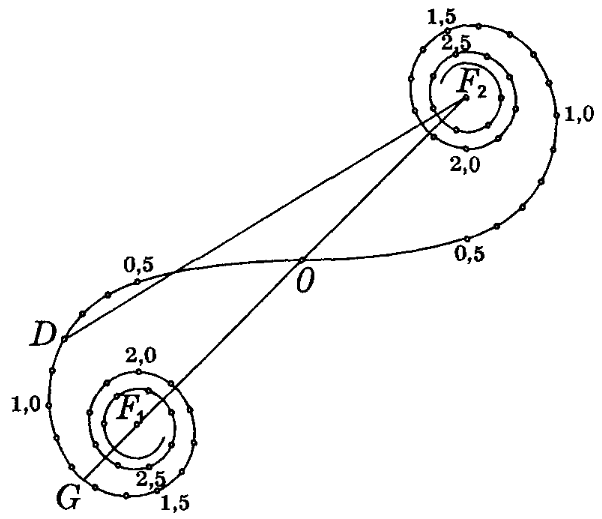
\includegraphics[scale=0.3]{figures/cornu}
\subsection{Фраунгофера}
\begin{gather*}
  \theta \approx 1.22 \frac{\lambda}{D}
\end{gather*}
На щели:
\begin{gather*}
  b\sim \theta_m = \pm m \lambda
\end{gather*}
где $b$ - ширина щели, $\theta_m$ - углы минимумов
\begin{gather*}
  A=A_0\frac{\sin(\delta/2)}{\delta/2} \qquad I=I_0 \frac{\sin^{2}\alpha}{\alpha^{2}} \\ 
  \alpha = \frac{\delta}{2} = \frac{\pi \Delta}{\lambda} = \frac{\pi b \sin \theta}{\lambda}
\end{gather*}
Если волна под углом $\theta_0$ к нормали:
\begin{gather*}
  \Delta = b (\sin \theta_m - \sin \theta_0) = \pm m \lambda 
\end{gather*}
\subsection{Решётка}
\begin{gather*}
  I=I_1N^{2} \qquad d\sin \theta_m = \pm m \lambda
\end{gather*}
N - кол-во щелей, b - ширина одной щели, d - расстояние между, $\theta_m$ - главные минимумы

При наклоне $d(\sin \theta_m - \sin \theta_0)=\pm m \lambda$
\begin{gather*}
  I=I_0 \frac{\sin^{2}(\delta/2)}{(\delta/2)^{2}} \frac{\sin^{2}(N\gamma/2)}{\sin^{2}(\gamma/2)} \\ 
  \delta = 2\pi b \sin \frac{\theta}{\lambda} \qquad \gamma = 2 \pi d \sin \frac{\theta}{\lambda}
\end{gather*}
Угловая дисперсия $\frac{d\theta}{d\lambda}=\frac{m}{d\cos \theta}$

Разрешающая способность $R=\lambda/\delta \lambda = m N$

Область дисперсии $\Delta \lambda = \lambda / m$
\section{Поляризация}
Закон Малюса: $I=I_0\cos^{2}\phi$

Угол Брюстера: $\tan \theta=n_2/n_1$

Формулы Френеля, коэффициенты отражения для линейного поляризованного света 
относительно плоскости падения, $\theta_1$ - угол падения, $\theta_2$ - угол преломления:
\begin{gather*}
  \rho_{\perp}=\frac{\sin^{2}(\theta_1-\theta_2)}{\sin^{2}(\theta_1+\theta_2)} \qquad \rho_{\parallel}=\frac{\tan^{2}(\theta_1-\theta_2)}{\tan^{2}(\theta_1+\theta_2)}
\end{gather*}
Фазовая пластинка: $h = \frac{\Delta \phi \lambda}{2\pi \Delta n}$
\section{Дисперсия}
\begin{gather*}
  v_{\text{gr}}=v_{\text{ph}}-\lambda \frac{d v_{\text{ph}}}{d\lambda}  \\ 
  v_{gr}=\frac{d\omega}{dk}
\end{gather*}
Плазма: $n^{2}=1-(\frac{\omega_{pl}}{\omega})^{2}$, газ: $n^{2}=1+\frac{\omega_{pl}^{2}}{\omega_0^{2}-\omega^{2}}$

Закон Бугера: $I=I_0 e^{-\kappa x}$

Закон Релея: $I \sim \omega^{4}$
\section{Волновод}
\begin{gather*}
  \nu_{cr}=\frac{c_0}{2}\sqrt{(m/a)^{2}+(n/b)^{2}} \qquad TE_{mn} \\ 
  v_{gr}=c_0\sqrt{1-(\omega_{cr}/\omega)^{2}} \qquad v_{gr}v_{ph}=c_0^{2} \\ 
  \lambda=\frac{\lambda_{\text{волн}\lambda_{cr}}}{\sqrt{\lambda_{\text{волн}^{2}+\lambda_{cr}^{2}}}}
\end{gather*}
\section{Интерферометр Фабри-Перо}
\[
  \nu = \frac{c}{2L}
\]
- расстояние между модами
\section{Уширение}
Ударное из уравнения неопределённости и длины свободного пробега ($d$ порядка $10^{-10}$ м): 
\begin{gather*}
  \Delta \nu_{imp}=\frac{1}{2\pi \tau} \qquad \tau=\frac{1}{n\sigma \bar{v}} \qquad n =\frac{P}{kt} \qquad \sigma=\pi d^{2}
\end{gather*}
Доплера:
\begin{gather*}
  \frac{\Delta \lambda_{dp}}{\lambda}=\frac{v}{c}
\end{gather*}
\section{Тепловое излучение}
\begin{gather*}
  I=\epsilon\sigma T^{4} \qquad \sigma=5.67 \cdot 10^{-8} \\ 
  \lambda^{*}=\frac{b}{T} \qquad b = 2.9 \cdot 10^{-3} \\ 
\end{gather*}

\end{document}

